\chapter{Tracking student progress using linked NAPLAN data} \label{chap4}

\section{Introduction}

The Victorian cohort that sat NAPLAN in \mbox{Year 3} in 2009 did \mbox{Year 9} NAPLAN in 2015. They provide a rich source of data to track progress over six years of schooling. Our methodology analyses this cohort in two different ways:
\begin{itemize}
\item by student background (parental education, school advantage, geolocation of school)
\item by NAPLAN score in \mbox{Year 3}.\footnote{We classify students according to the 20th, 50th, and 80th percentiles of Victorian performance, which we refer to as `low, medium, and high' \mbox{Year 3} score respectively.}
\end{itemize}
When tracking results and progress, we report the progress made by the median student within each sub-group, or for the median student starting from a given percentile. While results are reported in terms of \textit{equivalent year levels} and \textit{years of progress}, the analysis takes place using simulated NAPLAN scale scores and gain scores; only at the very last step are these results converted to equivalent year levels.\footnote{Because our results are based on percentiles, the results would not change if the simulated NAPLAN scale scores were converted to equivalent year levels before undergoing the analysis presented in this section. However, if the results were based around the \textit{means} of different sub-groups, these would change if the simulated NAPLAN scale scores were converted to equivalent year levels before undergoing analysis.}   

\section{Estimating median NAPLAN scale scores}

\subsection{By student background} \label{sec:ses_sub}

For each sub-group, we estimate the NAPLAN scale score (for each of numeracy and reading) and the corresponding equivalent year level of the median student in Years 3, 5, 7, and 9. The obvious way to do this is via the sample median in each year level, but this approach could lead to progress being overstated for some sub-groups. This is because there are more missing data in higher year levels, due to greater levels of absenteeism and withdrawal, as well as students who leave Victoria. As Section \ref{sec:missing} shows, students from households with lower parental education typically score below average, are more likely to miss a NAPLAN test, and typically make smaller gains than other students after controlling for prior NAPLAN score. This implies that the median student that sat a particular NAPLAN test in \mbox{Year 9} is likely to have scored above the observed median student when they took the test in \mbox{Year 3}.\footnote{If all students took all tests, we would expect the median \mbox{Year 3} student to match up to the median \mbox{Year 9} student.}

It is difficult to account for all the bias due to missing data, but we take an approach to estimating median scores that aims to reduce this bias. The sample median of each sub-group is used to estimate the population sub-group median in \mbox{Year 3}:
\begin{equation}
\widehat{Q_{50}\left[X_{j,3}|s\right]} = \tilde{x}_{j,3,s}
\end{equation}
Where $s$ is an indicator of sub-group.\footnote{See \Vref{chap3} for explanation of notation.} This is likely to be an overestimate of the population median for \mbox{Year 3}, given the patterns of missing data. But the proportion of missing data in \mbox{Year 3} is relatively small, meaning that the bias is likely to be small.

For Years 5, 7, and 9, we define a function for the median sub-group NAPLAN score conditional on \mbox{Year 3} score:
\begin{equation} \begin{array}{c}
Q_{50}\left[X_{j,Y}|s,X_{j,3}\right] = h_{j,Y,s}\left(X_{j,3}\right) \\
Y = 5,7,9
\end{array} \end{equation}
The functions $h_{j,Y,s}$ are estimated for $j = $ reading and numeracy, $Y = 5, 7, 9$, and for each subgroup using least absolute deviations. Restricted cubic regression splines are used to allow for non-linearity in $h_{j,Y,s}$. These functions are evaluated at the estimated \mbox{Year 3} sample median for each sub-group, $\tilde{x}_{j,3,s}$, to estimate each sub-group population medians for Years 5, 7, and 9:
\begin{equation} \begin{array}{c}
\widehat{Q_{50}\left[X_{j,Y}|s\right]} = \widehat{h}_{j,y,s}\left(\tilde{x}_{j,3,s}\right) \\
Y = 5,7,9
\end{array} \end{equation}
These estimates are typically lower than the sample medians in \mbox{Year 9}, suggesting that this approach reduces some of the bias due to missing data.\footnote{This approach is still likely to overestimate the sub-group medians, since excluding missing data is likely to overstate gain scores, as evidenced by \Vref{fig:missing}.}

\newpage
\subsection{Estimating percentiles}

We estimate the 20th, 50th, and 80th percentiles for the population in \mbox{Year 3}:
\begin{equation} \begin{array}{c}
\widehat{Q_{20}\left[X_{j,3}\right]} = \tilde{x}^{(20)}_{j,3} \\
\widehat{Q_{50}\left[X_{j,3}\right]} = \tilde{x}^{(50)}_{j,3} \\
\widehat{Q_{80}\left[X_{j,3}\right]} = \tilde{x}^{(80)}_{j,3}
\end{array} \end{equation}
These are used to track progress within each sub-group (and for the population) for a given achievement level in \mbox{Year 3}. We estimate the median NAPLAN score in Years 5, 7, and 9 conditional on sub-group \textit{and} \mbox{Year 3} percentile:
\begin{equation} \begin{array}{c}
\widehat{Q_{50}\left[X_{j,Y}|s,X_{j,3}\right]} = \widehat{h}_{j,y,s}\left(\tilde{x}^{(P)}_{j,3}\right) \\
Y = 5,7,9
\end{array} \end{equation}
where $P$ represents the \mbox{Year 3} percentile, and $\widehat{h}_{j,y,s}$ has been estimated separately for each year level and sub-group.\footnote{While $\widehat{h}_{j,y,s}$ is estimated separately for different sub-groups, it is not estimated separately for different percentiles.}

This means that for every sub-group, we have estimated median NAPLAN scale scores in Years 3, 5, 7, and 9, both for the median of the sub-group, and conditional on the \mbox{Year 3} percentile for the Victorian population. \Cref{tab:below_dip} shows these results for students who do not have a parent with a degree or diploma. Given this is a disadvantaged sub-group, the group median results are, unsurprisingly, lower than the results for the 50th percentile of the Victorian population in \mbox{Year 3}.

\begin{table}[H]
  \centering
  \captionwithunits{For each sub-group we estimate both group medians and the medians conditional on \mbox{Year 3} percentile}{Estimated median NAPLAN scale score, parental education below diploma, Victorian 2009--15 cohort}

    \begin{tabular}{lcrrr}
          &       & \multicolumn{3}{c}{Year 3 percentile} \\

          & \multicolumn{1}{c}{Group median} & \multicolumn{3}{c}{(Victorian population)} \\     \cmidrule(lr){3-5}
    Year level & (below diploma) & \multicolumn{1}{c}{20th} & \multicolumn{1}{c}{50th} & \multicolumn{1}{c}{80th} \\ \midrule
    Year 3 & \multicolumn{1}{c}{390.7} & 344.5 & 408.9 & 476.9 \\
    Year 5 & \multicolumn{1}{c}{477.0} & 452.4 & 487.1 & 526.2 \\
    Year 7 & \multicolumn{1}{c}{520.8} & 496.9 & 530.4 & 570.6 \\
    Year 9 & \multicolumn{1}{c}{570.6} & 549.4 & 579.3 & 615.3 \\
    \bottomrule
    \end{tabular}%
  \label{tab:below_dip}%
\begin{flushleft}\source{Grattan analysis of \textcite{vcaa2015}.}\end{flushleft}
\vspace{-15pt}
\end{table}%


\section{Converting NAPLAN scale scores to equivalent year levels}

Having estimated a range of NAPLAN scale scores for sub-groups, it is then possible to convert these to equivalent year levels. As outlined in Section \ref{sec:theoretical}, every NAPLAN scale score within the range of the median student between \mbox{Year 1} and \mbox{Year 13} has a corresponding equivalent year level. Having estimated a function that maps NAPLAN scale scores onto equivalent year levels, $Y^{*} = \widehat{f}_{j}^{-1}\left(X_{j}\right)$, it is straightforward to find the equivalent year level corresponding to the NAPLAN scale point estimates. The reported equivalent year level includes both the schooling year and any additional months of learning.\footnote{We divide each year of learning into twelve months. An alternative approach that other grade-equivalent scales have taken is to divide a year of learning into ten months, noting that the school year is roughly ten months long.}

Years (and months) of progress between Years 3 and 9 for a particular sub-group is then calculated as the difference in equivalent year levels between Years 3 and 9. The median student is expected to make six years of progress over this time.

\section{Robustness of student progress results} \label{sec:robust_progress}

\subsection{Confidence intervals for student progress}

As outlined in Section \ref{sec:pv}, 99 per cent confidence intervals are calculated for estimates of student progress using a bootstrap simulation. This takes into account uncertainty arising from estimation of equivalent year levels, as well as uncertainty around estimates of student progress.

\Cref{fig:pct_ci} gives an example showing that point estimates of equivalent year levels for sub-groups are typically estimated within three months of the upper and lower confidence bounds. These are relatively narrow confidence intervals, which can be attributed to the large sample size of each sub-group analysed.

When estimating years of progress for different sub-groups from the same percentile in \mbox{Year 3}, statistical significance is implied by confidence intervals that do not overlap. As shown in \Cref{fig:par_ed_ss_ci}, confidence intervals do not overlap for different levels of parental education from the same \mbox{Year 3} score, implying that parental education is statistically significant. Full results for reading and numeracy with confidence bounds are available for download from the Grattan Institute website.\footnote{\url{http://grattan.edu.au/report/widening-gaps/}}

\begin{figure}[H]
 \captionwithunits{The 99 per cent confidence intervals for large sub-groups are typically less than $\pm$ three months}{Estimated equivalent year level by highest level of parental education, reading, Victorian 2009--15 cohort}
 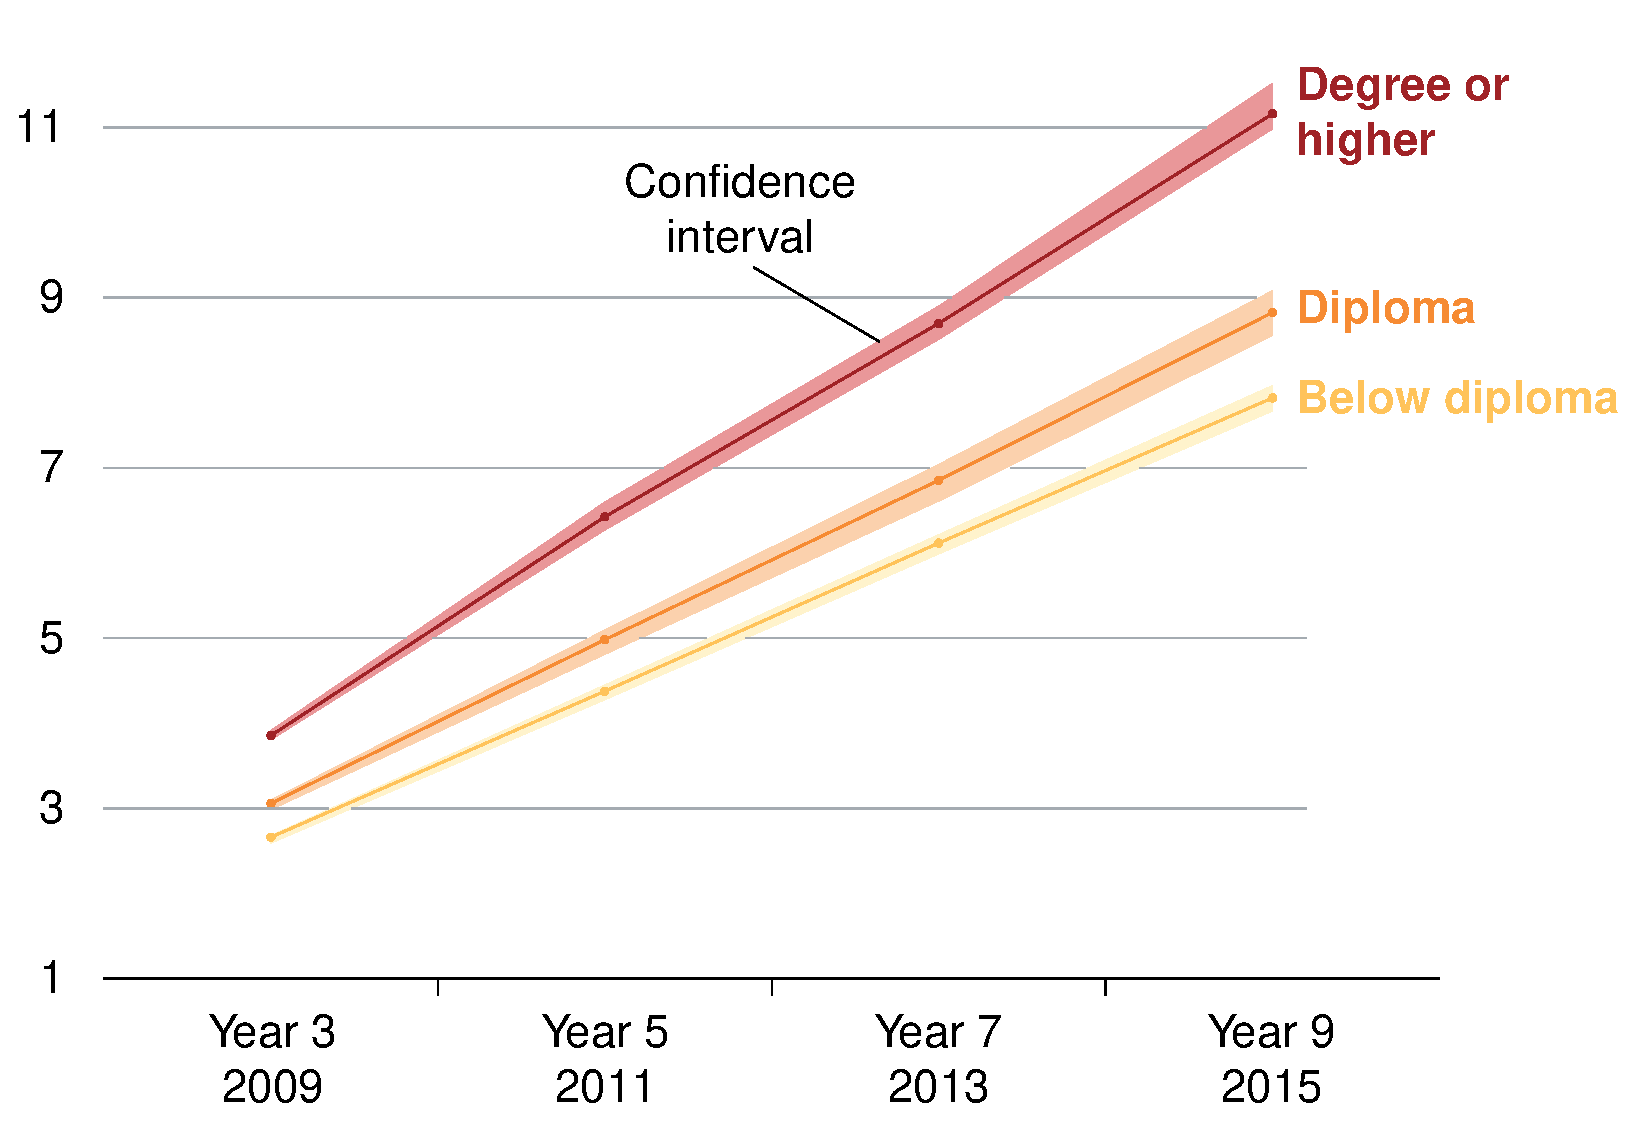
\includegraphics[width=\columnwidth]{atlas/pct_ci.pdf}\label{fig:pct_ci}
\notes{Chart shows 99 per cent confidence interval}

\source{Grattan analysis of \textcite{vcaa2015,acara2014}.}
\end{figure}

\begin{figure}[H]
 \captionwithunits{Confidence intervals suggest that parental education is significant in explaining student progress}{Estimated years of progress by highest level of parental education, numeracy, Victorian 2009--15 cohort}
 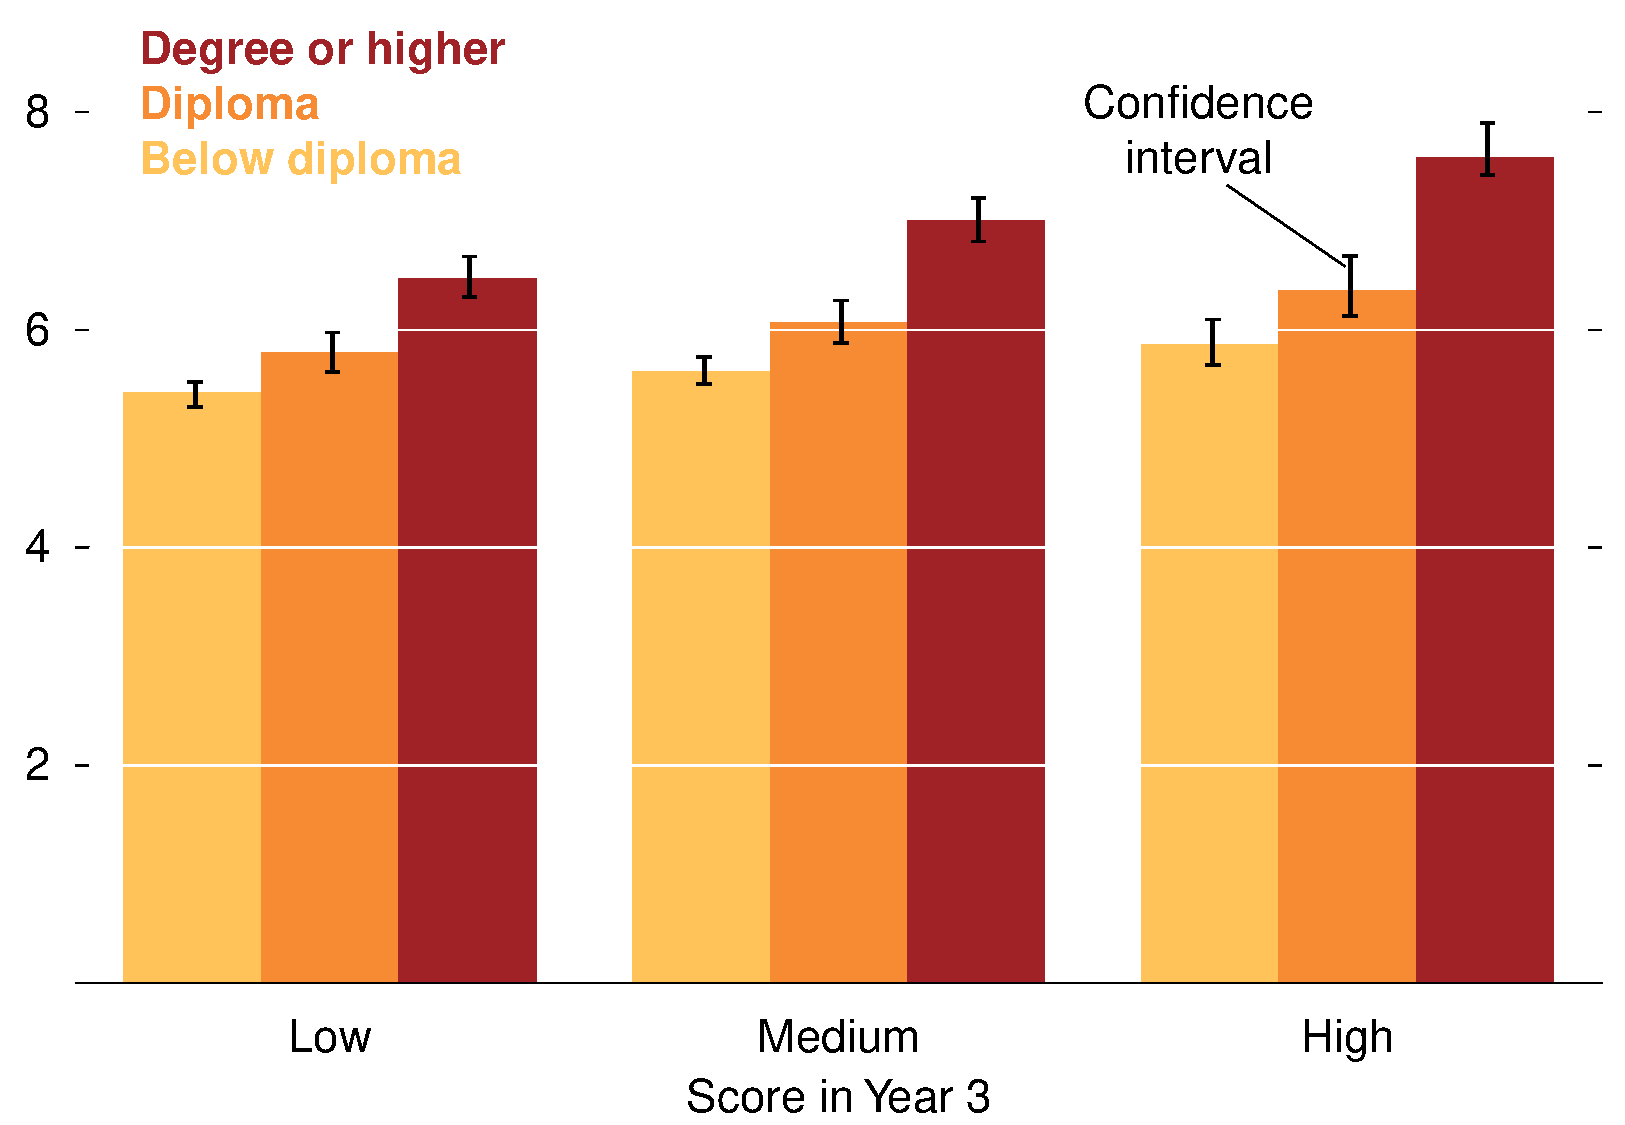
\includegraphics[width=\columnwidth]{atlas/par_ed_ss_ci.pdf}\label{fig:par_ed_ss_ci}

\notes{`Low, medium and high' score in \mbox{Year 3} refers to the 20th, 50th and 80th percentiles for the Victorian population. Chart shows 99 per cent confidence interval}

\source{Grattan analysis of \textcite{vcaa2015,acara2014}.}
\end{figure}

\newpage
\subsection{Impact of regression to the mean on estimated gaps} \label{sec:reg_mean_gaps}

Section \ref{sec:rttm} discussed the problem of \textit{regression to the mean}, where a student with an extreme score on one test is likely to be closer to the average score on the next test. While we were not able to correct for this in our analysis, we aimed to keep any bias arising to a minimum by avoiding extreme percentiles in our analysis.

Nonetheless, when comparing years of progress for a given \mbox{Year 3} score, regression to the mean may lead to overestimation of the gaps between different sub-groups. At the 20th percentile in \mbox{Year 3} (for the Victorian population), the score is more extreme for students with a university-educated parent than for those without. The \mbox{Year 9} score for students with the university-educated parent will regress towards the mean score of this group, which is higher than the mean score of students without a university-educated parent. Similarly, at the 80th percentile in \mbox{Year 3}, the score is more extreme for students where no parent has a degree or diploma -- the \mbox{Year 9} score for these students will regress towards a lower mean than for other students.

\newpage
We do not believe that regression to the mean explains a significant proportion of the estimated gaps between students from households where a parent has a university degree, and those from households where no parent has a degree or diploma. For students who score at the 50th percentile in \mbox{Year 3}, this is relatively close to the group mean for all categories of parental education, meaning that regression to the mean will have a very small effect. Yet we still estimate a significant gap between the parental education categories `degree or higher' and `below diploma', consistent with the gaps found at the 20th and 80th percentiles.\footnote{The estimated gap is larger at the 80th percentile, and smaller at the 20th percentile.}

We also estimate years of progress conditional on the 20th, 50th and 80th percentiles \textit{within} each parental education sub-group. Although this means we are comparing students from different starting scores, we would not expect regression to the mean to impact the estimated gaps in progress between these groups, since the within-group percentiles are as extreme as each other. As \Cref{fig:gaps_pc} shows, the gaps in progress estimated between `degree or higher' and `below diploma' are just as high as those estimated from the 20th, 50th and 80th percentiles for the Victorian population; they are, in fact, between one and two months of learning larger.

\begin{figure}[H]
 \captionwithunits{Comparing years of progress from within-group percentiles does not reduce gaps between parental education groups}{Estimated years of progress by highest level of parental education, numeracy, Victorian 2009--15 cohort}
 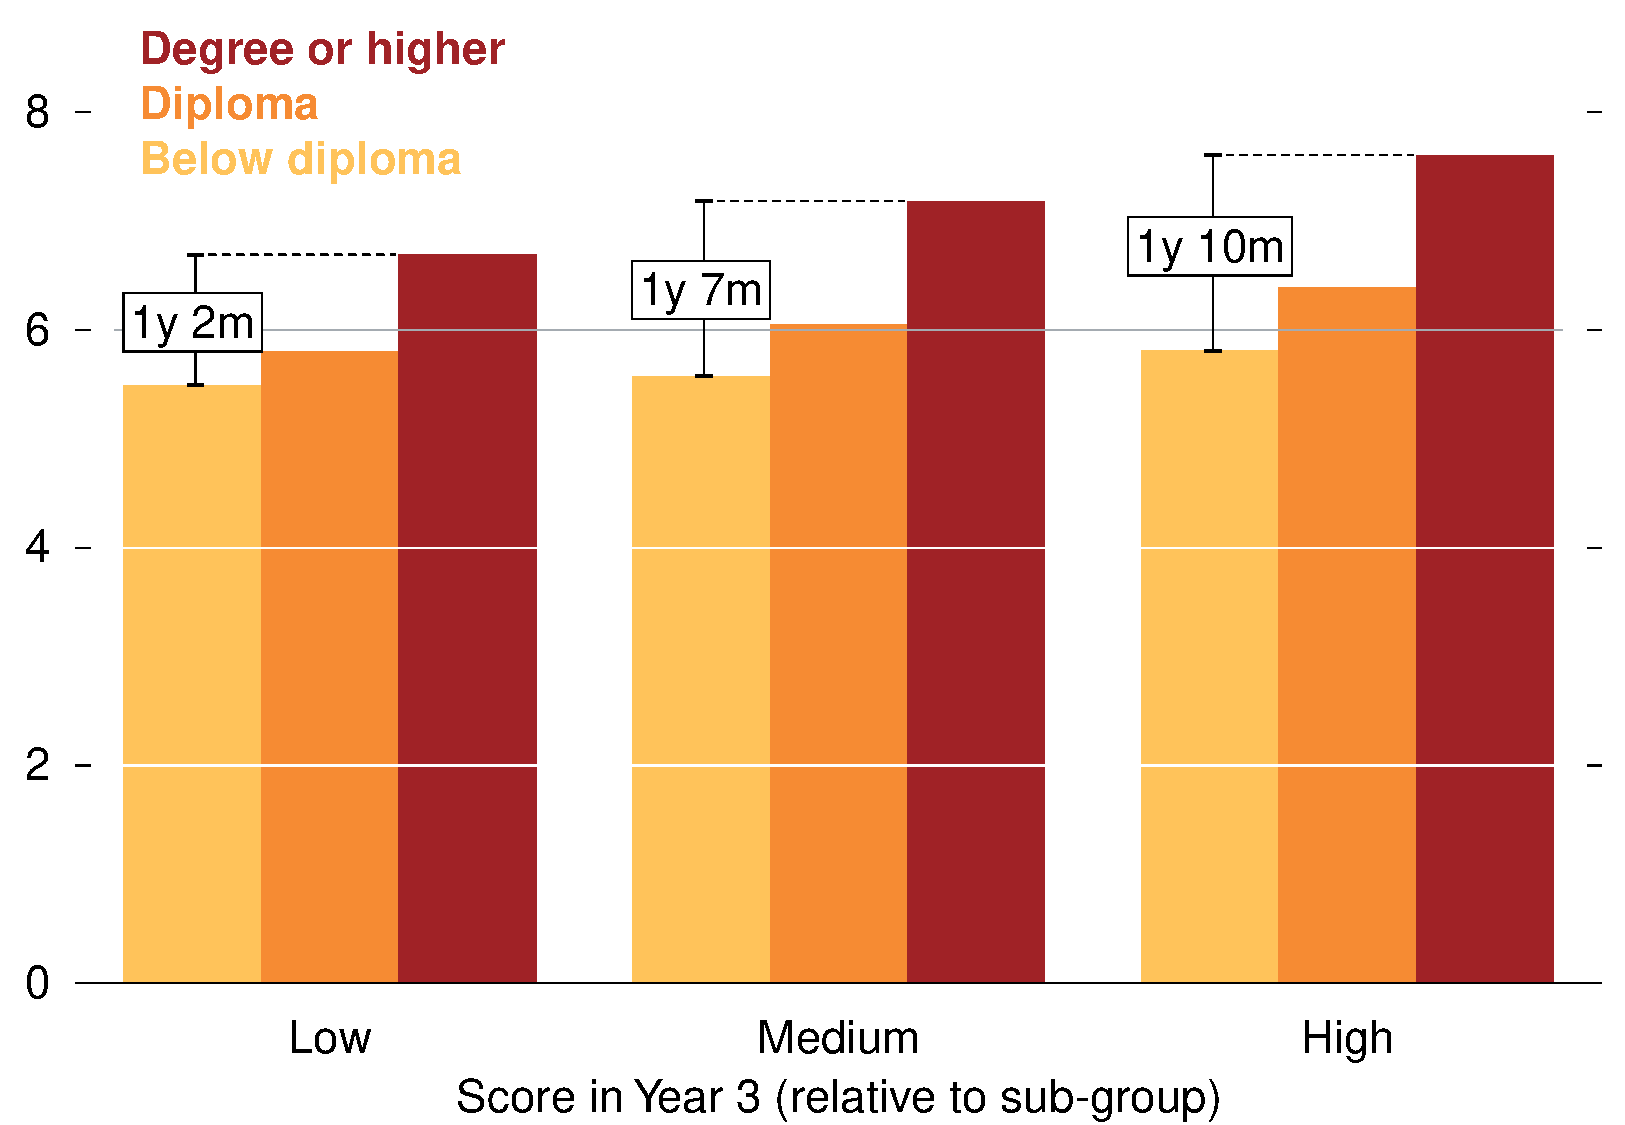
\includegraphics[width=\columnwidth]{atlas/gaps_pc.pdf}\label{fig:gaps_pc}
\notes{`Low, medium and high' score in \mbox{Year 3} refers to the 20th, 50th and 80th percentiles within each sub-group (as opposed to \Cref{fig:par_ed_ss_ci} which is based on percentiles for the Victorian population).}

\source{Grattan analysis of \textcite{vcaa2015,acara2014}.}
\end{figure}

\newpage
\subsection{Robustness of results to the cohort analysed} \label{sec:cohort2}

\textit{Widening gaps} reports student progress based on an analysis of the cohort of Victorian students that sat the \mbox{Year 3} NAPLAN tests in 2009, and the \mbox{Year 9} tests in 2015. It is important to validate the results using another cohort, to see if the key conclusions are specific to this particular cohort.

We also have linked data available for the cohort of Victorian students that sat the \mbox{Year 3} NAPLAN tests in 2008, and the \mbox{Year 9} tests in 2014. \Cref{fig:par_ed_08,fig:par_ed_ss_08} show that the results for different sub-groups of parental education are similar across the 2008--14 and the 2009--15 cohorts, with similar gaps in student progress opening between high and low levels of parental education. However, there are differences. \mbox{Year 3} students at the 20th percentile in numeracy in 2009 are estimated to make about five additional months of progress over six years as their counterparts at the 20th percentile in 2008.

We do not interpret this to mean that low achievers in the 2009 cohort made better learning progress than low achievers in the 2008 cohort. In particular, the differences may be the result of equating error or some other factor. Rather, we interpret the broad consistency of findings between the two cohorts to mean that the key findings in \textit{Widening gaps} are sufficiently robust to inform policy decisions.\footnote{Results are not shown for every sub-group analysed in the report, but the patterns of results based on the 2008--14 cohort are consistent with those for the 2009--15 cohort.}

\begin{figure}[H]
 \captionwithunits{Both Victorian cohorts estimate similar levels for parental education sub-groups}{Estimated equivalent year level by highest year of parental education, reading, Victoria}
 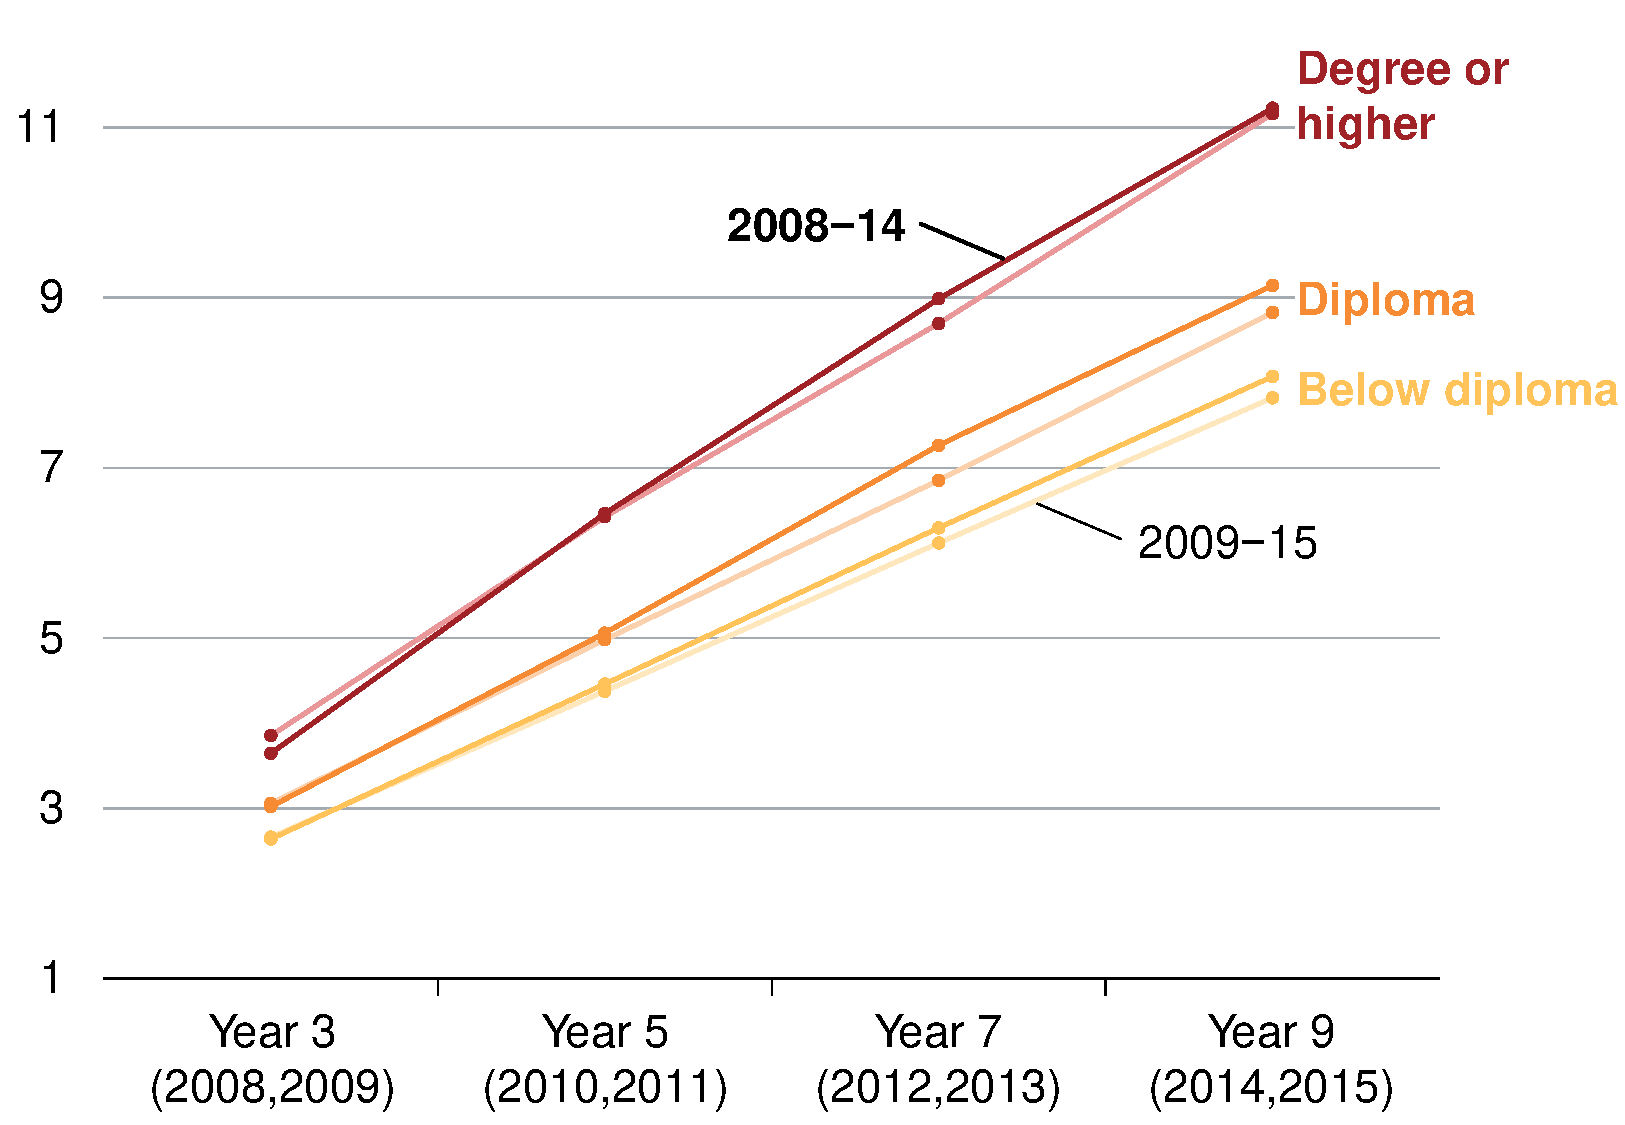
\includegraphics[width=\columnwidth]{atlas/par_ed_08.pdf}\label{fig:par_ed_08}

\source{Grattan analysis of \textcite{vcaa2014,vcaa2015,acara2014}.}
\end{figure}

\begin{figure}[H]
 \captionwithunits{Both Victorian cohorts estimate similar gaps in progress by parental education and \mbox{Year 3} score}{Estimated years of progress by highest level of parental education, numeracy, Victoria}
 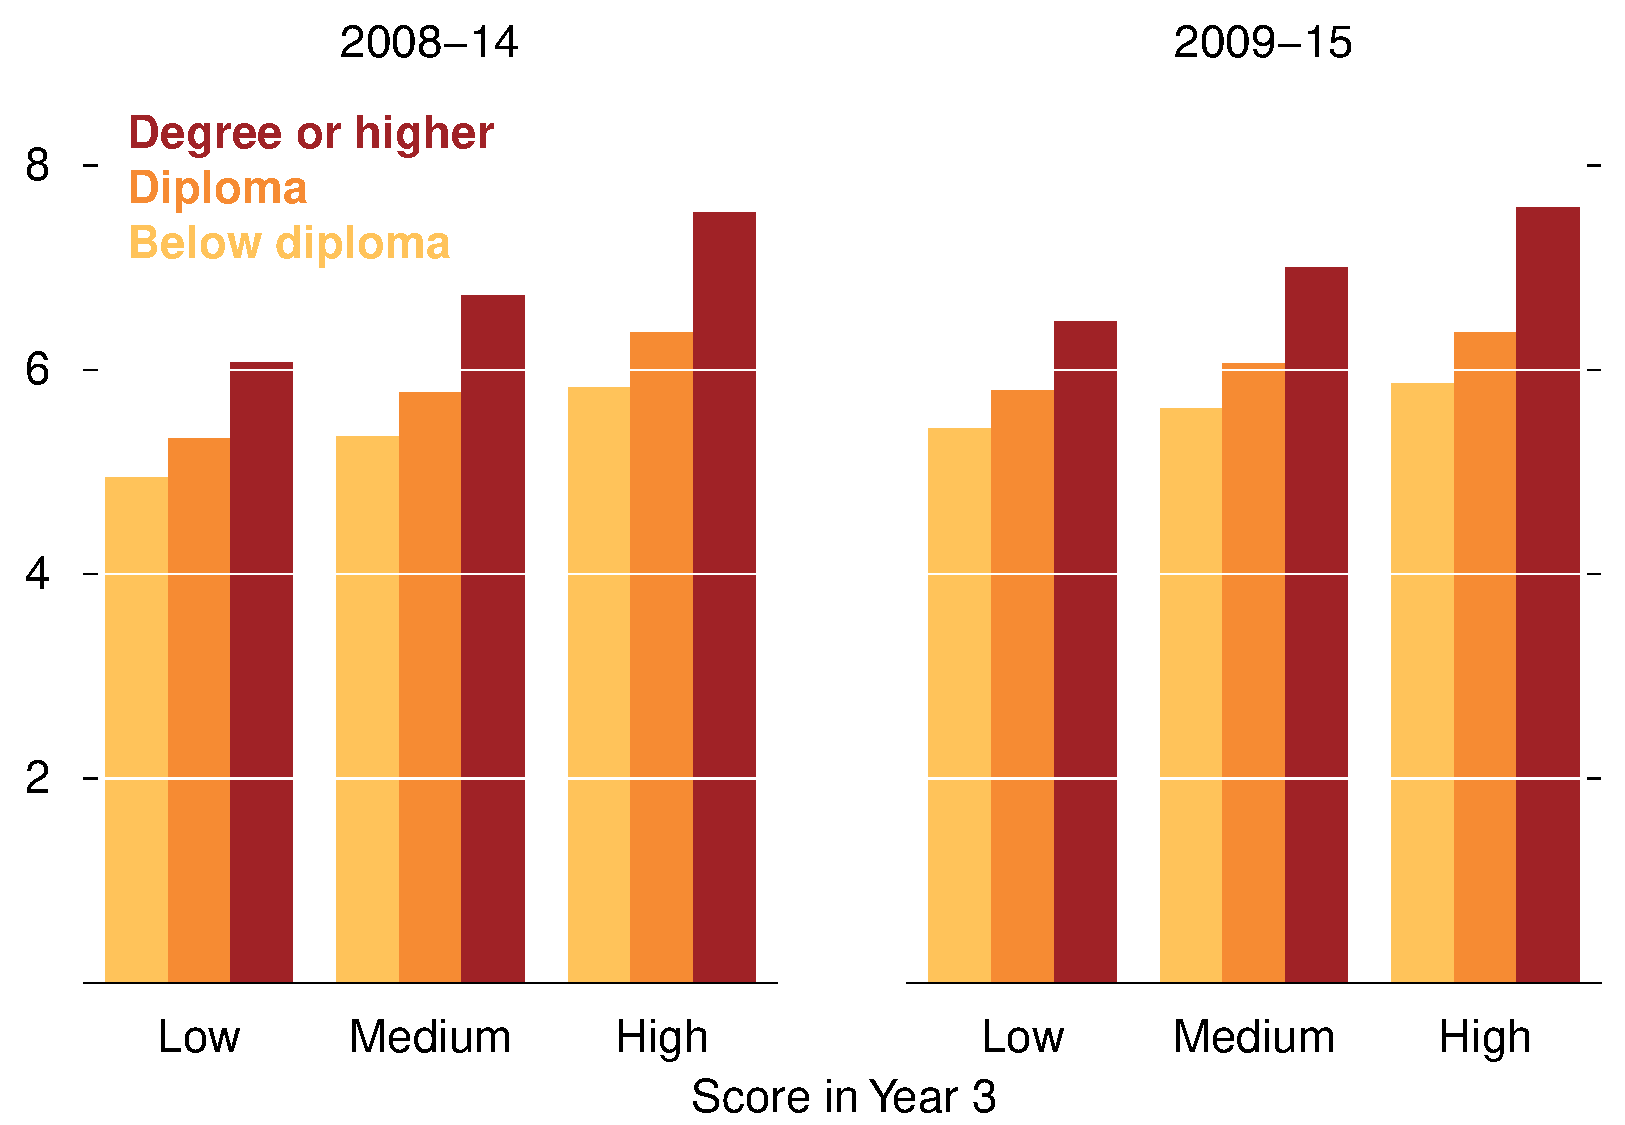
\includegraphics[width=\columnwidth]{atlas/par_ed_ss_08.pdf}\label{fig:par_ed_ss_08}
 \notes{`Low, medium and high' score in \mbox{Year 3} refers to the 20th, 50th and 80th percentiles for the Victorian population.}

\source{Grattan analysis of \textcite{vcaa2014,vcaa2015,acara2014}.}
\end{figure}